\subsubsection{Logistic Regression Results}
\label{sec:logistic_regression_results}

As part of the machine learning baseline models evaluated in this study, a Logistic Regression classifier was implemented and trained on the preprocessed dataset. This linear model, commonly used for binary classification tasks, is known for its simplicity, interpretability, and solid performance in high-dimensional spaces such as textual data. The model yielded promising results on the test set, achieving an \textbf{accuracy} of 0.8627, a \textbf{precision} of 0.8980, a \textbf{recall} of 0.8246, and an \textbf{F1-score} of 0.8597. These metrics indicate a balanced performance in detecting both hate and non-hate speech categories, demonstrating the classifier's effectiveness even when compared with more complex deep learning approaches. In terms of interpretability and computational efficiency, Logistic Regression remains a reliable and practical choice for deployment in moderation systems.

\begin{figure}[H]
    \centering
    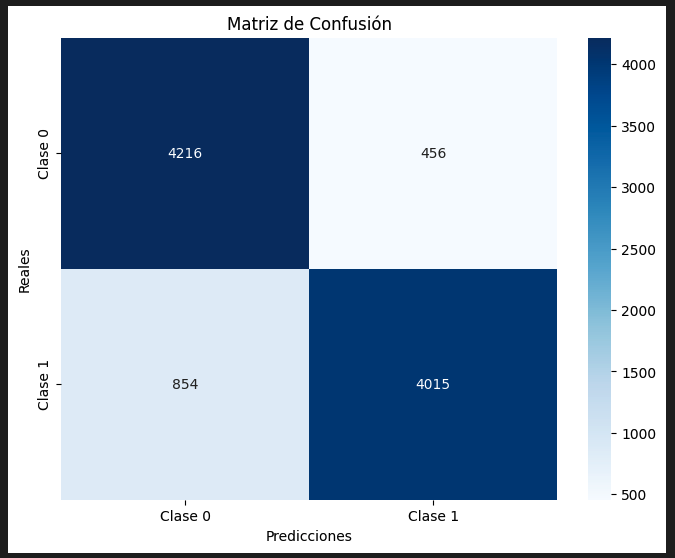
\includegraphics[width=0.7\linewidth]{images/confusion_matrix_logisticregression.png} 
    \caption{Confusion matrix of the Logistic Regression model.}
    \label{fig:confusion_matrix_logistic_regression}
\end{figure}

The logistic regression model demonstrates good performance, with precision close to 90\% and recall of 82.5\%, correctly classifying the majority of cases. Although there are some false negatives, the balance between precision and recall is adequate, indicating that the model is reliable for the task but could be adjusted if reducing a specific type of error is desired.